% SAGE: Smart Agentic-Guided Empowerment
% arXiv preprint — uses standard article class with minimal dependencies
% Compile: pdflatex sage.tex && bibtex sage && pdflatex sage.tex && pdflatex sage.tex

\documentclass[11pt,a4paper]{article}

% --- Packages ---
\usepackage[utf8]{inputenc}
\usepackage[T1]{fontenc}
\usepackage{lmodern}
\usepackage[margin=1in]{geometry}
\usepackage{amsmath,amssymb}
\usepackage{graphicx}
\usepackage{booktabs}
\usepackage{hyperref}
\usepackage{xcolor}
\usepackage{algorithm}
\usepackage{algorithmic}
\usepackage{enumitem}
\usepackage{caption}
\usepackage{subcaption}
\usepackage{tikz}
\usetikzlibrary{shapes,arrows,positioning,fit,calc,backgrounds,decorations.pathreplacing}
\usepackage{listings}
\usepackage{natbib}
\usepackage{url}
\usepackage{multirow}

% --- Hyperref setup ---
\hypersetup{
    colorlinks=true,
    linkcolor=blue!60!black,
    citecolor=blue!60!black,
    urlcolor=blue!60!black
}

% --- Code listing style ---
\lstset{
    basicstyle=\ttfamily\small,
    breaklines=true,
    frame=single,
    numbers=left,
    numberstyle=\tiny\color{gray},
    keywordstyle=\color{blue!70!black},
    commentstyle=\color{green!50!black},
    stringstyle=\color{red!60!black},
    showstringspaces=false,
    tabsize=2
}

% --- Title ---
\title{
    \textbf{SAGE: Smart Agentic-Guided Empowerment} \\[0.5em]
    \large A Governance-First Multi-Agent Framework for Regulated Industries
}

\author{
    Suman Shetty H \\
    \texttt{github.com/Sumanharapanahalli/SAGE} \\
    \texttt{MIT License}
}

\date{April 2026}

\begin{document}

\maketitle

% ============================================================================
\begin{abstract}
We present SAGE (Smart Agentic-Guided Empowerment), an open-source, modular multi-agent orchestration framework designed for regulated industries where auditability, human oversight, and compliance are non-negotiable. Unlike existing frameworks (LangGraph, CrewAI, AutoGen) that treat human approval as optional per-node configuration, SAGE enforces a two-tier governance architecture: framework control operations execute immediately, while all agent proposals require mandatory human-in-the-loop (HITL) approval with immutable audit trails and trace-level accountability.

SAGE introduces several novel contributions: (1)~a YAML-first declarative agent manifest system enabling domain-agnostic configuration without code changes; (2)~a Build Orchestrator implementing eight agentic patterns including EMA-based adaptive routing and N-provider multi-critic review; (3)~an Agent Gym training engine with Glicko-2 skill ratings, spaced repetition, and Best-First Tree Search (BFTS) for solution-space exploration; (4)~eleven domain-specific execution runners spanning software, firmware, PCB design, ML, and documentation; (5)~a Product Owner agent converting basic customer inputs into structured requirements following proper product management principles; (6)~a comprehensive Systems Engineering framework implementing IEEE 15288 standards with regulatory compliance (IEC 62304, 21 CFR Part 11); (7)~OpenTelemetry distributed tracing and CloudEvents structured messaging for observability; (8)~a pluggable Connector Framework for external data source integration (GitHub, filesystem); (9)~complexity-based model routing that classifies prompt difficulty and routes to cost-appropriate LLM providers; (10)~SQLite-backed persistent stores for chat conversations and OKR goals; (11)~zero mandatory API keys enabling fully air-gapped deployment; (12)~a multi-standard compliance verification engine covering IEC 62304, ISO 26262, DO-178C, EN 50128, and 21 CFR Part 11; and (13)~a compliance engineering suite including bidirectional traceability matrices, HMAC-signed audit chains, change control workflows, and regulatory document generation.

The system comprises ${\sim}100{,}000$ lines of production code (77K Python + 23K TypeScript), 250+ REST API endpoints, 34 React UI pages, and 17 modular skills, including comprehensive regulatory compliance capabilities. Empirical evaluation across 618 Agent Gym training sessions demonstrates measurable skill improvement (average Glicko-2 rating: 1,492), while a 100-solution stress test reveals current scaling limitations (2\% end-to-end success rate) with documented root cause analysis. We report both successes and failures transparently.

\medskip
\noindent\textbf{Keywords:} multi-agent systems, human-in-the-loop, regulated AI, lean development, agent training, governance
\end{abstract}

% ============================================================================
\section{Introduction}
\label{sec:intro}

The rapid proliferation of large language model (LLM)-powered agent frameworks has produced increasingly capable systems for task decomposition, code generation, and autonomous decision-making~\citep{yao2023react, shinn2023reflexion, hong2023metagpt}. However, the current generation of open-source frameworks --- LangGraph~\citep{langgraph2024}, CrewAI~\citep{crewai2024}, AutoGen~\citep{wu2023autogen}, Semantic Kernel~\citep{semantickernel2024}, and Dify~\citep{dify2024} --- share a common architectural assumption: agent output can be acted upon immediately, with human inspection occurring post-hoc via execution logs.

This assumption fails catastrophically in regulated industries. Medical device development (ISO~13485, IEC~62304), automotive systems (ISO~26262), financial services (SOC~2, PCI~DSS), and aerospace software (DO-178C) require provable human oversight for every consequential decision. The question is not ``does the system work?'' but rather \textit{``can you prove it worked correctly, with human oversight, for every decision?''}

No existing open-source framework provides the combination of:
\begin{itemize}[noitemsep]
    \item Mandatory human approval gates (not optional per-node configuration)
    \item Immutable per-decision audit trails with trace identifiers
    \item Rejection feedback loops that improve future agent behavior
    \item Domain-agnostic YAML-only configuration for new industries
    \item Zero mandatory API keys (fully air-gappable deployment)
\end{itemize}

SAGE addresses this gap by applying lean development methodology~\citep{poppendieck2003lean} to multi-agent orchestration: eliminate waste, shorten feedback loops, and amplify human judgment at machine speed. The framework's north-star design principle is enabling one human operator supported by an AI agent team to manage operations that traditionally require large teams --- but only with governance guarantees sufficient for regulated environments.

\subsection{Contributions}

This paper makes the following contributions:

\begin{enumerate}[noitemsep]
    \item \textbf{Two-tier governance architecture} separating immediate framework control from approval-gated agent proposals, with risk-classified proposals and trace-level audit trails (\S\ref{sec:governance}).

    \item \textbf{Build Orchestrator} implementing eight agentic patterns --- ReAct, hierarchical decomposition, wave-based parallelism, EMA-based adaptive routing, N-provider multi-critic review, HITL gates, iterative refinement, and anti-drift checkpoints --- for end-to-end product construction (\S\ref{sec:orchestrator}).

    \item \textbf{Agent Gym} training engine with Glicko-2 skill ratings, spaced repetition scheduling, BFTS tree search~\citep{aiscientistv2}, and adaptive exercise selection across 661 seed exercises in 11 domains (\S\ref{sec:gym}).

    \item \textbf{Domain-aware runner architecture} with eleven specialized execution environments implementing a common \texttt{BaseRunner} interface (\S\ref{sec:runners}).

    \item \textbf{Modular skill marketplace} with 17 YAML-based skill manifests supporting public, private, and disabled visibility tiers (\S\ref{sec:skills}).

    \item \textbf{Communication layers} comprising OpenTelemetry distributed tracing with graceful no-op degradation and CloudEvents v1.0 structured messaging (\S\ref{sec:communication}).

    \item \textbf{Connector Framework} providing pluggable external data source integration via an abstract base connector with registry pattern, shipping GitHub and filesystem connectors (\S\ref{sec:connectors}).

    \item \textbf{Complexity-based model routing} that heuristically classifies prompt difficulty and routes to cost-appropriate LLM providers (\S\ref{sec:routing}).

    \item \textbf{Empirical evaluation} across 618 training sessions and 100-solution stress tests with transparent reporting of both successes and failures (\S\ref{sec:evaluation}).
\end{enumerate}

% ============================================================================
\section{Related Work}
\label{sec:related}

\paragraph{Multi-Agent Frameworks.}
LangGraph~\citep{langgraph2024} provides a graph-based orchestration model with optional \texttt{interrupt\_before} nodes for human intervention --- a partial HITL mechanism, but not mandatory or audited. CrewAI~\citep{crewai2024} introduces role-based agent hierarchies with delegation but lacks structured audit trails. AutoGen~\citep{wu2023autogen} supports multi-agent conversations with code execution sandboxing. MetaGPT~\citep{hong2023metagpt} assigns agents SOPs (Standard Operating Procedures) modeled on software company roles. None enforce mandatory governance across all agent actions or provide domain-agnostic YAML-only configuration.

\paragraph{Agent Training and Evaluation.}
AlphaCode~\citep{li2022alphacode} and AlphaCode~2~\citep{leblond2023alphacode2} demonstrate competitive programming via large-scale sampling and filtering. SWE-Bench~\citep{jimenez2024swebench} evaluates agents on real GitHub issues. AgentBench~\citep{liu2023agentbench} provides multi-environment benchmarks. These are static benchmarks. SAGE's Agent Gym differs by implementing continuous Glicko-2~\citep{glickman2001glicko2} rating with spaced repetition~\citep{leitner1972} for progressive skill development: agents improve over time through repeated practice, not one-shot evaluation.

\paragraph{Human-in-the-Loop AI.}
Constitutional AI~\citep{bai2022constitutional} and RLHF~\citep{ouyang2022rlhf} incorporate human feedback during model training. Interactive machine learning~\citep{amershi2014power} enables runtime human guidance. SAGE's approach is distinct: human feedback at the \textit{proposal level} (not the training level) is stored in vector memory and used to improve future proposals without model retraining, following the Memento principle~\citep{memento2025}.

\paragraph{Lean Development and AI.}
Lean software development~\citep{poppendieck2003lean} emphasizes eliminating waste, building quality in, and deferring commitment. SAGE applies these principles to agent orchestration: the five-phase lean loop (Surface $\rightarrow$ Contextualize $\rightarrow$ Propose $\rightarrow$ Decide $\rightarrow$ Compound) eliminates manual steps while preserving human judgment at decision points.

\paragraph{Governance in AI Systems.}
The EU AI Act~\citep{euaiact2024} and FDA AI/ML guidance~\citep{fdaaiml2023} establish regulatory requirements for AI systems in high-risk applications. Paperclip~\citep{paperclip2024} implements board-of-directors governance targeting eventual zero-human operation. SAGE takes the opposite stance: human approval is permanent, not transitional, reflecting the requirements of regulated industries where full autonomy is neither permitted nor desirable.

% ============================================================================
\section{System Architecture}
\label{sec:architecture}

\subsection{Design Principles}

SAGE is built on five foundational laws:

\begin{enumerate}[noitemsep]
    \item \textbf{Agents propose, humans decide} --- for all agent proposals. Framework control operations (configuration, LLM switching) execute immediately as operator actions.
    \item \textbf{Eliminate waste at every layer} --- no manual steps that an agent can perform correctly; no ceremonies that don't add value.
    \item \textbf{Compounding intelligence over cold-start lookup} --- every human correction feeds vector memory, improving future proposals without model retraining.
    \item \textbf{Vertical slices, not horizontal layers} --- every task produces a complete, reviewable end-to-end slice of value.
    \item \textbf{Atomic verification is non-negotiable} --- every agent action has a defined verification step.
\end{enumerate}

\subsection{Architecture Overview}

Figure~\ref{fig:architecture} illustrates SAGE's layered architecture.

\begin{figure}[h]
\centering
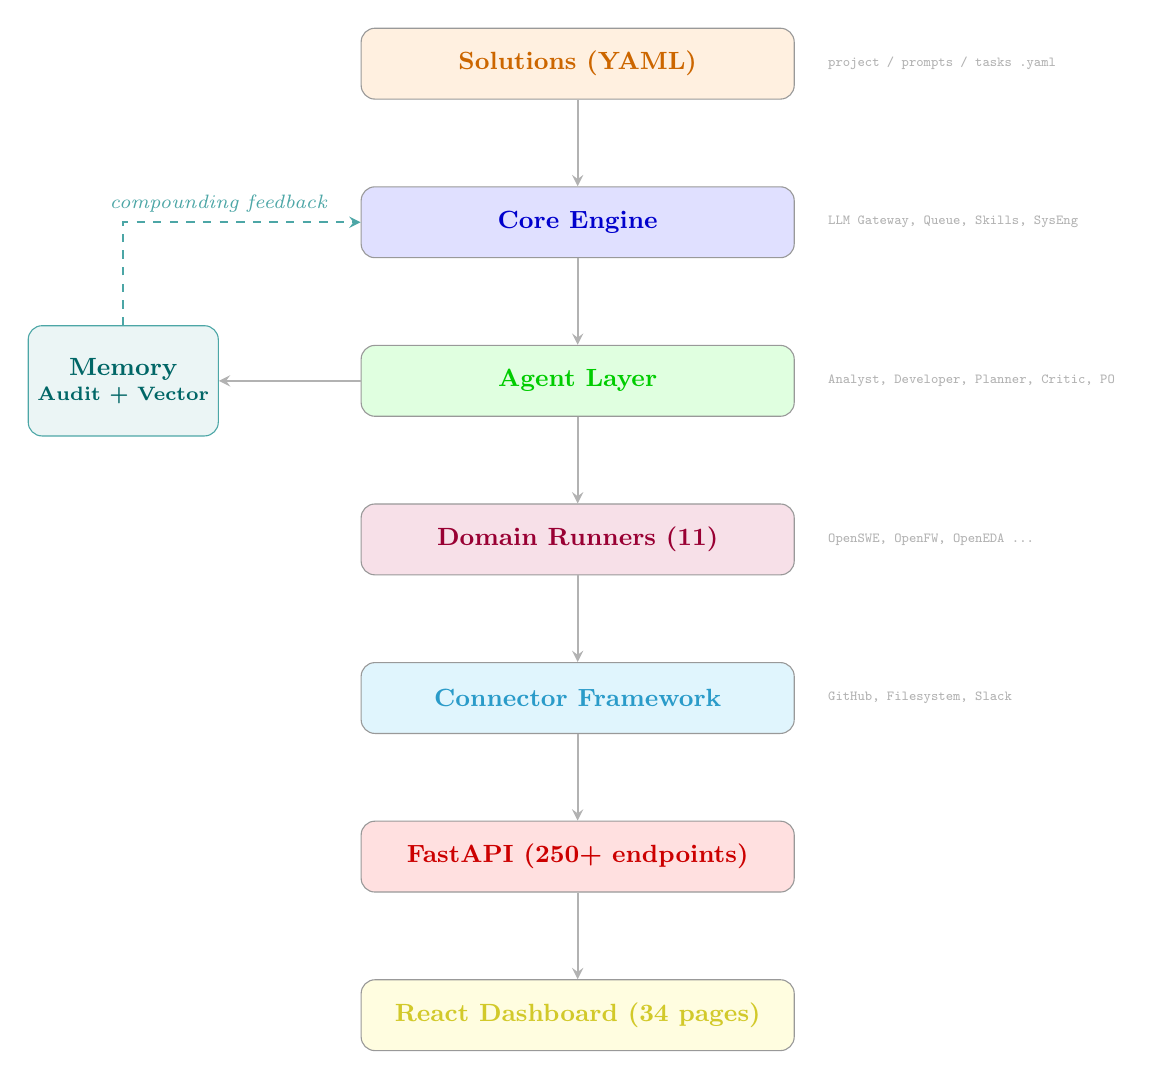
\begin{tikzpicture}[
    node distance=1.1cm,
    layer/.style={rectangle, draw=gray!80, rounded corners=5pt, minimum width=5.5cm, minimum height=0.9cm, font=\small\bfseries, fill=#1!12, text=#1!80!black},
    layer/.default=blue,
    annot/.style={font=\tiny\ttfamily, text=gray!60, anchor=west},
    arrow/.style={->, thick, >=stealth, color=gray!60},
    darrow/.style={->, thick, >=stealth, dashed, color=teal!70}
]
    % Layers — centered stack
    \node[layer=orange]                   (sol)     {Solutions (YAML)};
    \node[layer=blue,    below=of sol]    (core)    {Core Engine};
    \node[layer=green,   below=of core]   (agents)  {Agent Layer};
    \node[layer=purple,  below=of agents] (runners) {Domain Runners (11)};
    \node[layer=cyan,    below=of runners](conn)    {Connector Framework};
    \node[layer=red,     below=of conn]   (api)     {FastAPI (250+ endpoints)};
    \node[layer=yellow,  below=of api]    (ui)      {React Dashboard (34 pages)};

    % Right-side annotations
    \node[annot, right=0.3cm of sol.east]     {project / prompts / tasks .yaml};
    \node[annot, right=0.3cm of core.east]    {LLM Gateway, Queue, Skills, SysEng};
    \node[annot, right=0.3cm of agents.east]  {Analyst, Developer, Planner, Critic, PO};
    \node[annot, right=0.3cm of runners.east] {OpenSWE, OpenFW, OpenEDA \ldots};
    \node[annot, right=0.3cm of conn.east]    {GitHub, Filesystem, Slack};

    % Memory — left side
    \node[rectangle, draw=teal!70, rounded corners=5pt, minimum width=2cm, minimum height=1.4cm,
          fill=teal!8, font=\small\bfseries, text=teal!80!black, align=center,
          left=1.8cm of agents] (memory) {Memory\\[-2pt]{\scriptsize Audit + Vector}};

    % Downward arrows
    \draw[arrow] (sol)     -- (core);
    \draw[arrow] (core)    -- (agents);
    \draw[arrow] (agents)  -- (runners);
    \draw[arrow] (runners) -- (conn);
    \draw[arrow] (conn)    -- (api);
    \draw[arrow] (api)     -- (ui);

    % Memory feedback loop
    \draw[arrow] (agents.west) -- (memory.east);
    \draw[darrow] (memory.north) |- node[above, pos=0.7, font=\scriptsize\itshape, color=teal!70] {compounding feedback} (core.west);

\end{tikzpicture}
\caption{SAGE dependency hierarchy. Solutions plug in via YAML only. The Connector Framework provides pluggable external data source integration. The API exposes agents, runners, and connectors to the UI. The dashed arrow represents the compounding feedback loop: human decisions stored in memory enrich future agent context.}
\label{fig:architecture}
\end{figure}

The framework enforces strict separation between the \textit{framework} (\texttt{src/}, \texttt{web/}) and \textit{solutions} (\texttt{solutions/<name>/}). The framework is domain-agnostic; solutions encode all industry-specific knowledge via three YAML files:

\begin{itemize}[noitemsep]
    \item \texttt{project.yaml} --- declarative agent manifest (what this domain \textit{is})
    \item \texttt{prompts.yaml} --- role definitions and system prompts (how agents \textit{think})
    \item \texttt{tasks.yaml} --- task type registry (what agents \textit{can do})
\end{itemize}

Adding a new industry domain requires editing only these three YAML files. No Python code changes are needed.

\subsection{LLM Gateway}
\label{sec:llm}

The \texttt{LLMGateway} provides a unified interface across six provider backends:

\begin{table}[h]
\centering
\caption{Supported LLM providers. All except Claude API work without API keys.}
\label{tab:providers}
\begin{tabular}{lll}
\toprule
\textbf{Provider} & \textbf{Setup} & \textbf{API Key Required} \\
\midrule
Gemini CLI & \texttt{npm install -g @google/gemini-cli} & No \\
Claude Code CLI & \texttt{npm install -g @anthropic-ai/claude-code} & No \\
Ollama & \texttt{ollama serve \&\& ollama pull llama3.2} & No \\
Local (GGUF) & \texttt{pip install llama-cpp-python} + model & No \\
Generic CLI & Any CLI tool via \texttt{generic\_cli\_path} & No \\
Claude API & \texttt{ANTHROPIC\_API\_KEY} env var & Yes \\
\bottomrule
\end{tabular}
\end{table}

The gateway is a singleton with a thread lock ensuring single-lane inference. Provider switching is available at runtime via \texttt{POST /llm/switch} without server restart. OpenTelemetry spans wrap every \texttt{generate()} call with GenAI semantic conventions (\S\ref{sec:communication}).

% ============================================================================
\section{Two-Tier Governance Architecture}
\label{sec:governance}

SAGE's central design contribution is the separation of operations into two governance tiers:

\begin{table}[h]
\centering
\caption{Two-tier governance. Framework control executes immediately; agent proposals require human approval.}
\label{tab:governance}
\begin{tabular}{lll}
\toprule
\textbf{Tier} & \textbf{Operations} & \textbf{Behavior} \\
\midrule
Framework Control & \texttt{config\_switch}, \texttt{llm\_switch}, \texttt{module\_toggle} & Immediate execution \\
Agent Proposals & \texttt{yaml\_edit}, \texttt{code\_diff}, \texttt{agent\_hire}, ... & HITL approval required \\
\bottomrule
\end{tabular}
\end{table}

Figure~\ref{fig:governance} illustrates the two-tier split.

\begin{figure}[h]
\centering
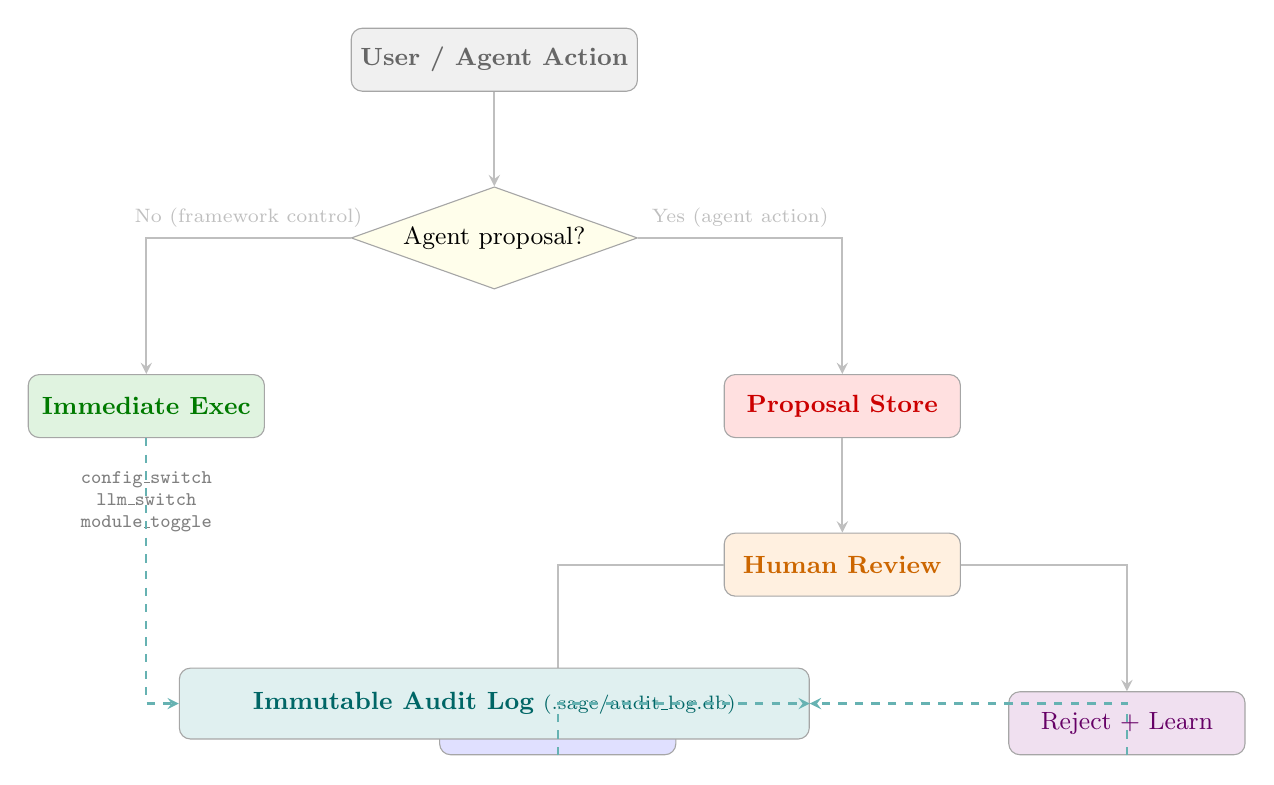
\begin{tikzpicture}[
    box/.style={rectangle, draw=gray!70, rounded corners=4pt, minimum width=3cm, minimum height=0.8cm, font=\small, fill=#1!12, text=#1!80!black},
    box/.default=blue,
    arr/.style={->, thick, >=stealth, color=gray!50},
    node distance=1cm and 2cm
]
    % Input
    \node[box=gray, minimum width=3.5cm] (action) {\textbf{User / Agent Action}};

    % Decision diamond
    \node[diamond, draw=gray!70, below=1.2cm of action, aspect=2.8, fill=yellow!8, font=\small, inner sep=2pt] (check) {Agent proposal?};

    % Two branches
    \node[box=green!60!black, below left=1.4cm and 2cm of check] (immediate) {\textbf{Immediate Exec}};
    \node[box=red, below right=1.4cm and 2cm of check] (proposal) {\textbf{Proposal Store}};

    % Downstream — framework ops
    \node[below=0.3cm of immediate, font=\scriptsize\ttfamily, text=gray, align=center] (imm_list) {config\_switch\\llm\_switch\\module\_toggle};

    % Downstream — HITL path
    \node[box=orange, below=1.2cm of proposal] (hitl) {\textbf{Human Review}};
    \node[box=blue, below left=1.2cm and 0.6cm of hitl] (approve) {Execute};
    \node[box=violet, below right=1.2cm and 0.6cm of hitl] (reject) {Reject + Learn};

    % Arrows
    \draw[arr] (action) -- (check);
    \draw[arr] (check) -| node[above, pos=0.25, font=\scriptsize] {No (framework control)} (immediate);
    \draw[arr] (check) -| node[above, pos=0.25, font=\scriptsize] {Yes (agent action)} (proposal);
    \draw[arr] (proposal) -- (hitl);
    \draw[arr] (hitl) -| (approve);
    \draw[arr] (hitl) -| (reject);

    % Audit log — full width at bottom
    \node[box=teal, below=4.8cm of check, minimum width=8cm, minimum height=0.9cm]
        (audit) {\textbf{Immutable Audit Log} {\scriptsize (.sage/audit\_log.db)}};
    \draw[arr, dashed, color=teal!60] (approve.south) |- (audit);
    \draw[arr, dashed, color=teal!60] (reject.south) |- (audit);
    \draw[arr, dashed, color=teal!60] (immediate.south) |- (audit);

\end{tikzpicture}
\caption{Two-tier governance flow. Framework control operations execute immediately; agent proposals are held for human review. Both paths write to the immutable audit log.}
\label{fig:governance}
\end{figure}

\subsection{Product Owner Agent}
\label{sec:product-owner}

The Product Owner agent (\texttt{src/agents/product\_owner.py}) addresses the requirements engineering gap where customers provide vague descriptions ("I want a fitness app") and expect developers to infer complete product specifications. Instead of requiring customers to write perfect product requirements documents, the agent conducts structured interviews following proper product management principles.

The agent implements a three-phase workflow: (1)~\textbf{Analysis} --- evaluates customer input completeness across seven dimensions (clarity, user focus, value proposition, scope, success metrics, technical constraints, business context); (2)~\textbf{Clarification} --- generates 3-5 smart questions using the 5W1H method (Who, What, When, Where, Why, How) to fill knowledge gaps; and (3)~\textbf{Backlog Creation} --- synthesizes gathered information into structured product backlogs with user personas, INVEST-compliant user stories, MoSCoW prioritization, and acceptance criteria.

The output format follows industry standards: user stories in "As a [persona], I want [capability] so that [benefit]" format, acceptance criteria with testable conditions, and story point estimates for development planning. This eliminates the common failure mode where development teams guess at product intent from incomplete specifications.

\subsection{Systems Engineering Framework}
\label{sec:systems-engineering}

The Systems Engineering framework (\texttt{src/core/systems\_engineering.py}) implements IEEE 15288 standards with full regulatory compliance for industries requiring formal systems engineering processes (medical devices, automotive, aerospace). The framework provides five core capabilities:

\textbf{Requirements Traceability:} Four bidirectional matrices ensure complete coverage: User Needs $\rightarrow$ System Requirements $\rightarrow$ Design Architecture $\rightarrow$ Verification Activities $\rightarrow$ Validation Evidence. Each matrix tracks completeness percentages and identifies traceability gaps.

\textbf{V-Model Implementation:} Structured decomposition following the systems engineering V-model with verification at each level. Requirements are classified by type (functional, performance, interface, safety, security, usability, reliability, maintainability, compliance) and allocated to appropriate subsystems.

\textbf{Change Control:} Formal change management per IEC 62304 §6.1 with impact assessment, approval workflows, and complete audit trails. Changes are assessed for regression risk, testing impact, and documentation requirements before execution.

\textbf{Electronic Signatures:} Full 21 CFR Part 11 compliance for regulatory submissions including signature workflows, integrity verification, signer identity validation, and complete audit trails for all signature activities.

\textbf{Regulatory Document Generation:} Automated creation of required regulatory deliverables including Software Requirements Specification (SRS), System Architecture Document (SAD), Verification \& Validation Plan, Risk Management File per ISO 14971, and SOUP (Software of Unknown Provenance) Inventory per IEC 62304 §7.1.

The framework provides automated compliance scoring with readiness levels (Audit Ready: 95\%+ traceability, Submission Ready: 80\%+, Development Ready: 60\%+) and gap analysis for regulatory submissions.

\subsection{Proposal Lifecycle}

Every agent proposal follows a structured lifecycle:

\begin{enumerate}[noitemsep]
    \item \textbf{Creation} --- Agent generates a proposal with a unique \texttt{trace\_id}, action type, and payload.
    \item \textbf{Risk Classification} --- Proposals are classified across five tiers: \textsc{Informational}, \textsc{Low}, \textsc{Medium}, \textsc{High}, and \textsc{Destructive}. Each tier has risk-appropriate expiry windows.
    \item \textbf{Review} --- Human reviews the proposal in the dashboard or via Slack integration.
    \item \textbf{Decision} --- Approval triggers execution via \texttt{ProposalExecutor}. Rejection with feedback stores the human's reasoning.
    \item \textbf{Compounding} --- Both approvals and rejections are indexed in vector memory, enriching future agent context.
\end{enumerate}

The immutable audit log (SQLite, per-solution isolation via \texttt{.sage/audit\_log.db}) records every event with timestamps, trace IDs, and decision metadata. This satisfies traceability requirements for IEC~62304, ISO~13485, and similar regulatory standards.

\subsection{The Lean Loop}

Every task processed by SAGE follows a five-phase compounding cycle:

\begin{equation}
\text{Surface} \rightarrow \text{Contextualize} \rightarrow \text{Propose} \rightarrow \text{Decide} \rightarrow \text{Compound}
\label{eq:lean-loop}
\end{equation}

Phase 5 (Compound) feeds back into Phase 2 (Contextualize) for subsequent tasks, as shown in Figure~\ref{fig:lean-loop}. The system improves with every human interaction through accumulated experience retrieval --- no model retraining required.

\begin{figure}[h]
\centering
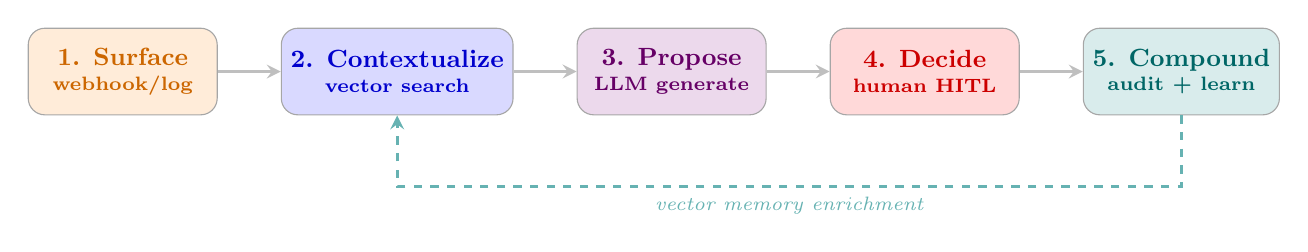
\begin{tikzpicture}[
    phase/.style={rectangle, draw=gray!70, rounded corners=6pt, minimum width=2.4cm, minimum height=1.1cm, font=\small\bfseries, fill=#1!15, text=#1!80!black, align=center},
    phase/.default=blue,
    arr/.style={->, very thick, >=stealth, color=gray!50},
    feedback/.style={->, very thick, >=stealth, dashed, color=teal!60},
    node distance=0.8cm
]
    % Phases in a row with good spacing
    \node[phase=orange]                     (surface)  {1. Surface\\[-2pt]{\scriptsize webhook/log}};
    \node[phase=blue,   right=of surface]   (context)  {2. Contextualize\\[-2pt]{\scriptsize vector search}};
    \node[phase=violet, right=of context]   (propose)  {3. Propose\\[-2pt]{\scriptsize LLM generate}};
    \node[phase=red,    right=of propose]   (decide)   {4. Decide\\[-2pt]{\scriptsize human HITL}};
    \node[phase=teal,   right=of decide]    (compound) {5. Compound\\[-2pt]{\scriptsize audit + learn}};

    % Forward arrows
    \draw[arr] (surface)  -- (context);
    \draw[arr] (context)  -- (propose);
    \draw[arr] (propose)  -- (decide);
    \draw[arr] (decide)   -- (compound);

    % Feedback loop: Compound → Contextualize (below, with generous vertical space)
    \draw[feedback] (compound.south) -- ++(0,-0.9) -| node[below, pos=0.25, font=\scriptsize\itshape, color=teal!60] {vector memory enrichment} (context.south);

\end{tikzpicture}
\caption{The SAGE Lean Loop. Every task follows five phases. The dashed arrow shows the compounding feedback path: human decisions in Phase~4 are indexed in vector memory, enriching the context retrieved in Phase~2 for subsequent tasks. No model retraining is required.}
\label{fig:lean-loop}
\end{figure}

% ============================================================================
\section{Build Orchestrator}
\label{sec:orchestrator}

The Build Orchestrator (\texttt{build\_orchestrator.py}, 2,878 lines) transforms plain-language product descriptions into structured codebases through eight integrated agentic patterns:

\subsection{Agentic Pattern Composition}

\begin{table}[h]
\centering
\caption{Eight agentic patterns in the Build Orchestrator.}
\label{tab:patterns}
\begin{tabular}{llp{6cm}}
\toprule
\textbf{\#} & \textbf{Pattern} & \textbf{Implementation} \\
\midrule
1 & ReAct & Per-task observe $\rightarrow$ think $\rightarrow$ act $\rightarrow$ observe loop \\
2 & Hierarchical Decomposition & LLM decomposes descriptions into task graphs (32 types) \\
3 & Wave-Based Parallelism & Independent tasks execute concurrently in waves \\
4 & EMA Adaptive Router & Exponential moving average score tracking per task-agent pair \\
5 & N-Provider Multi-Critic & Parallel review by $N$ LLM providers, weighted aggregation \\
6 & HITL Gates & Human sign-off at plan and integration stages \\
7 & Iterative Refinement & Critic score $<$ threshold triggers retry with feedback \\
8 & Anti-Drift Checkpoints & Crash recovery + quality degradation detection \\
\bottomrule
\end{tabular}
\end{table}

\subsection{Pipeline Stages}

The 0$\rightarrow$1 greenfield build pipeline proceeds through the states shown in Figure~\ref{fig:build-pipeline}.

\begin{figure}[h]
\centering
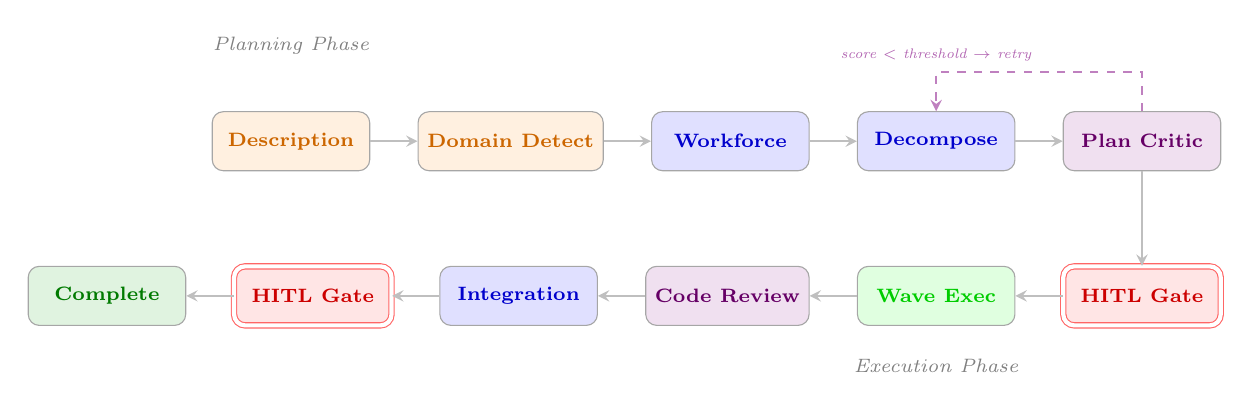
\begin{tikzpicture}[
    state/.style={rectangle, draw=gray!70, rounded corners=4pt, minimum width=2cm, minimum height=0.75cm, font=\scriptsize\bfseries, fill=#1!12, text=#1!80!black},
    state/.default=blue,
    hitl/.style={rectangle, draw=red!60, rounded corners=4pt, double, double distance=1.5pt, minimum width=2cm, minimum height=0.75cm, font=\scriptsize\bfseries, fill=red!10, text=red!80!black},
    arr/.style={->, thick, >=stealth, color=gray!50},
    critic/.style={->, thick, >=stealth, dashed, color=violet!50},
    node distance=0.5cm and 0.6cm
]
    % Row 1 — planning phase
    \node[state=orange]                      (desc)      {Description};
    \node[state=orange,  right=of desc]      (domain)    {Domain Detect};
    \node[state=blue,    right=of domain]    (workforce) {Workforce};
    \node[state=blue,    right=of workforce] (decomp)    {Decompose};
    \node[state=violet,  right=of decomp]    (critic1)   {Plan Critic};

    % Row 2 — execution phase (below, right-to-left)
    \node[hitl, below=1.2cm of critic1]      (hitl1)     {HITL Gate};
    \node[state=green,   left=of hitl1]      (waves)     {Wave Exec};
    \node[state=violet,  left=of waves]      (critic2)   {Code Review};
    \node[state=blue,    left=of critic2]    (integrate) {Integration};
    \node[hitl,          left=of integrate]  (hitl2)     {HITL Gate};

    % Final
    \node[state=green!60!black, left=of hitl2] (done) {Complete};

    % Row 1 arrows
    \draw[arr] (desc)      -- (domain);
    \draw[arr] (domain)    -- (workforce);
    \draw[arr] (workforce) -- (decomp);
    \draw[arr] (decomp)    -- (critic1);

    % Transition row 1 → row 2
    \draw[arr] (critic1.south) -- (hitl1.north);

    % Row 2 arrows (right to left)
    \draw[arr] (hitl1)     -- (waves);
    \draw[arr] (waves)     -- (critic2);
    \draw[arr] (critic2)   -- (integrate);
    \draw[arr] (integrate) -- (hitl2);
    \draw[arr] (hitl2)     -- (done);

    % Iterative refinement loop (above row 1)
    \draw[critic] (critic1.north) -- ++(0,0.5) -| node[above, pos=0.5, font=\tiny\itshape, color=violet!60] {score $<$ threshold $\rightarrow$ retry} (decomp.north);

    % Phase labels
    \node[above=0.6cm of desc, font=\scriptsize\itshape, color=gray] {Planning Phase};
    \node[below=0.3cm of waves, font=\scriptsize\itshape, color=gray] {Execution Phase};

\end{tikzpicture}
\caption{Build Orchestrator pipeline. Double-bordered nodes are HITL approval gates. The dashed arrow shows iterative refinement when critic score falls below threshold. Wave execution runs independent tasks in parallel.}
\label{fig:build-pipeline}
\end{figure}

Domain detection covers 13 industries via pattern-matched \texttt{DOMAIN\_RULES}, with workforce assembly from 19 agent roles across 5 teams defined in \texttt{WORKFORCE\_REGISTRY}.

\subsection{Adaptive Router}

The adaptive router maintains a score matrix $Q[\text{task\_type}][\text{agent\_role}]$ initialized uniformly. After each task completion with critic score $r \in [0, 100]$, the score is updated via exponential moving average:

\begin{equation}
Q[t][a] \leftarrow (1 - \alpha) \cdot Q[t][a] + \alpha \cdot r
\label{eq:router}
\end{equation}

where $\alpha = 0.3$ is the smoothing factor. The router selects the highest-scoring agent for each task type. While this resembles Q-learning in structure, it is a simplified variant without state transitions or the Bellman equation --- the ``state'' is simply the task type, and the ``action'' is the agent assignment. Despite this simplicity, the mechanism provides effective task-agent routing that compounds across builds.

\subsection{N-Provider Multi-Critic}

The \texttt{CriticAgent} supports $N$ LLM providers reviewing in parallel. Given scores $\{s_1, \ldots, s_N\}$ from providers with weights $\{w_1, \ldots, w_N\}$ (primary provider receives weight $1.5\times$):

\begin{equation}
s_{\text{agg}} = \frac{\sum_{i=1}^{N} w_i \cdot s_i}{\sum_{i=1}^{N} w_i}
\label{eq:critic}
\end{equation}

Disagreements exceeding 20 points from the mean are flagged. All individual assessments and flaws are merged and deduplicated.

% ============================================================================
\section{Agent Gym}
\label{sec:gym}

The Agent Gym implements a training engine where agents improve through structured practice, grading, and reflection. The design draws loosely from self-play training paradigms~\citep{silver2018alphazero, schrittwieser2020muzero} in the sense that agents learn from their own outputs, though the mechanism is fundamentally different: rather than tree search or learned models, SAGE agents use LLM-based reflection on critic feedback, with learnings stored in vector memory for retrieval in subsequent attempts.

\subsection{Training Loop}

Each training session executes a five-phase loop (Figure~\ref{fig:gym-loop}):

\begin{figure}[h]
\centering
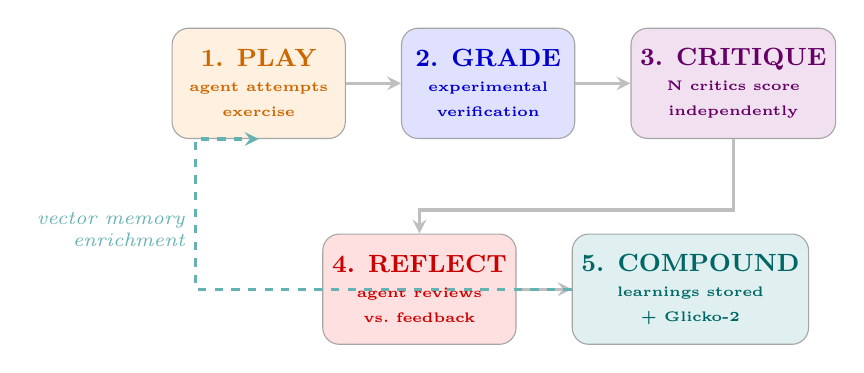
\begin{tikzpicture}[
    phase/.style={rectangle, draw=gray!70, rounded corners=6pt, minimum width=2.2cm, minimum height=1.4cm, font=\small\bfseries, fill=#1!12, text=#1!80!black, align=center},
    phase/.default=blue,
    arr/.style={->, very thick, >=stealth, color=gray!50},
    feedback/.style={->, very thick, >=stealth, dashed, color=teal!60},
    node distance=0.7cm
]
    % Top row: 3 phases
    \node[phase=orange]                   (play)     {1. PLAY\\[-2pt]{\tiny agent attempts}\\[-2pt]{\tiny exercise}};
    \node[phase=blue,   right=of play]    (grade)    {2. GRADE\\[-2pt]{\tiny experimental}\\[-2pt]{\tiny verification}};
    \node[phase=violet, right=of grade]   (critique) {3. CRITIQUE\\[-2pt]{\tiny N critics score}\\[-2pt]{\tiny independently}};

    % Bottom row: 2 phases (centered under the gap)
    \node[phase=red,  below right=1.2cm and -0.3cm of play]     (reflect)  {4. REFLECT\\[-2pt]{\tiny agent reviews}\\[-2pt]{\tiny vs.\ feedback}};
    \node[phase=teal, right=of reflect]   (compound) {5. COMPOUND\\[-2pt]{\tiny learnings stored}\\[-2pt]{\tiny + Glicko-2}};

    % Forward arrows
    \draw[arr] (play)     -- (grade);
    \draw[arr] (grade)    -- (critique);
    \draw[arr] (critique.south) |- ([yshift=0.3cm]reflect.north) -- (reflect.north);
    \draw[arr] (reflect)  -- (compound);

    % Feedback loop: Compound → Play
    \draw[feedback] (compound.west) -- ++(0,0) -| node[left, pos=0.7, font=\scriptsize\itshape, color=teal!60, align=right] {vector memory\\enrichment} ([xshift=-0.8cm]play.south) -- (play.south);

\end{tikzpicture}
\caption{Agent Gym training cycle. Phase~2 now includes experimental verification (real compilation, tests, simulation). Phase~5 stores reflections in vector memory, which enriches Phase~1 context in subsequent attempts. The Glicko-2 rating and spaced repetition schedule are updated at the end of each cycle.}
\label{fig:gym-loop}
\end{figure}

\begin{algorithm}[h]
\caption{Agent Gym Training Session}
\label{alg:gym}
\begin{algorithmic}[1]
\REQUIRE Agent role $r$, skill $s$, exercise $e$
\STATE $\text{attempt} \leftarrow \text{agent}(r).\text{execute}(e)$ \COMMENT{PLAY}
\STATE $\text{score} \leftarrow \text{runner}(s).\text{grade}(e, \text{attempt})$ \COMMENT{GRADE}
\STATE $\text{critiques} \leftarrow \text{multi\_critic}(\text{attempt}, e)$ \COMMENT{CRITIQUE}
\STATE $\text{reflection} \leftarrow \text{agent}(r).\text{reflect}(\text{attempt}, \text{critiques})$ \COMMENT{REFLECT}
\STATE $\text{vector\_store}.\text{add}(r, s, \text{reflection})$ \COMMENT{COMPOUND}
\STATE \text{update\_glicko2}(r, s, \text{score})
\IF{$\text{score} < \text{threshold}$}
    \STATE $\text{schedule\_spaced\_repetition}(e, \text{session\_count})$
\ENDIF
\end{algorithmic}
\end{algorithm}

\subsection{Glicko-2 Skill Ratings}

Each agent role $\times$ skill combination maintains a Glicko-2 rating triplet $(\mu, \phi, \sigma)$~\citep{glickman2001glicko2}:

\begin{itemize}[noitemsep]
    \item $\mu$ (rating): skill level, initialized at 1000, clamped $[100, 3000]$
    \item $\phi$ (rating deviation): confidence interval, starts at 350, minimum 30
    \item $\sigma$ (volatility): performance consistency
\end{itemize}

The 95\% confidence interval is $\mu \pm 2\phi$. Agents are considered deployment-ready when $\phi < 200$ (sufficient data for confident assessment). Note that combinations with few sessions ($<10$) may meet this threshold while still having high effective uncertainty; we report these transparently in our results.

\subsection{Spaced Repetition}

Failed exercises are scheduled for retry at increasing intervals following a modified Leitner system~\citep{leitner1972}:

\begin{equation}
\text{retry\_at} = \text{current\_session} + \{1, 3, 7, 15, 30\}[\min(\text{failure\_count} - 1, 4)]
\end{equation}

Exercises are cleared from the schedule upon successful completion.

\subsection{Adaptive Exercise Selection}

Exercise selection follows a three-tier priority system:

\begin{enumerate}[noitemsep]
    \item \textbf{Spaced repetition} --- failed exercises due for retry (highest priority)
    \item \textbf{Optimal zone} --- exercises with 40--70\% historical success rate (maximal learning)
    \item \textbf{Unseen} --- exercises not yet attempted (exploration)
\end{enumerate}

\subsection{Exercise Catalog}

The catalog contains 661 seed exercises across 11 domains (OpenSWE, OpenFW, OpenEDA, OpenSim, OpenML, OpenDoc, OpenDesign, OpenStrategy, OpenBrowser, OpenTerminal, AutoResearch), expandable to 50,000+ via LLM-generated variants along 10 axes per domain (platform, scale, constraint, compliance, etc.). The variant generation pipeline exists but has not been validated at scale beyond initial prototyping.

\subsection{Gym as Research Lab}
\label{sec:gym-lab}

A critical limitation of LLM-as-judge grading is that one language model evaluating another's text output provides no ground truth about whether the generated artifact \emph{actually works}. Code that ``looks correct'' to a critic may fail to compile. A circuit design that reads well may fail DRC checks. To address this, we introduce \textbf{experimental verification}: the gym executes generated artifacts in real toolchains and uses the execution results as the primary grading signal.

\subsubsection{Three-Tier Grading}

Grading combines three independent signals:

\begin{enumerate}[noitemsep]
    \item \textbf{Experimental execution (40\%)} --- the generated code is extracted, written to disk, and executed through domain-specific toolchains. Compilation success, test pass rates, and simulation outputs produce a deterministic score.
    \item \textbf{LLM critic review (30\%)} --- N independent LLM providers score the output semantically, now with experimental results included as context (e.g., ``pytest failed: 3/7 tests passing, AssertionError on line 42'').
    \item \textbf{Structural analysis (30\%)} --- fast pattern-based checks for code structure, error handling, and documentation.
\end{enumerate}

Each domain runner defines experimental verification commands specific to its toolchain:

\begin{table}[h]
\centering
\small
\caption{Per-runner experimental verification commands.}
\label{tab:exp-verify}
\begin{tabular}{@{}lll@{}}
\toprule
Runner & Verification Commands & Measures \\
\midrule
OpenSWE    & \texttt{py\_compile}, \texttt{pytest}, AST import & Syntax, test pass rate \\
OpenFW     & \texttt{gcc}, \texttt{arm-none-eabi-gcc}, \texttt{cppcheck} & Compilation, static analysis \\
OpenML     & \texttt{py\_compile}, training execution, \texttt{pytest} & Syntax, convergence, metrics \\
OpenEDA    & KiCad CLI netlist export, DRC & Schematic validity, rule violations \\
OpenDoc    & Markdown structure, \LaTeX{} structure & Heading count, section completeness \\
OpenDesign & SVG/XML parse, HTML parse, JSON validate & Artifact well-formedness \\
\bottomrule
\end{tabular}
\end{table}

\subsubsection{Critic-Refined Acceptance Criteria}

Static seed exercise criteria are necessary for bootstrapping but insufficient for sustained improvement. After two or more attempts at an exercise, the system invokes an LLM to \emph{refine acceptance criteria} based on accumulated experimental evidence. Criteria that are always trivially met are removed; criteria that experiments reveal as important but missing are added. Refined criteria are persisted in SQLite and used for subsequent sessions, creating a feedback loop where the definition of success evolves alongside agent capability.

\subsubsection{Human Expert Critic}

In addition to LLM critics, the system supports optional \textbf{human expert review}. Domain experts (mechanical engineers, firmware specialists, regulatory consultants) can review the same artifacts and experimental results that LLM critics see. Human reviews are queued asynchronously and, when submitted, are aggregated alongside LLM scores with $2\times$ weight. This reflects the higher reliability of expert judgment for domain-specific quality assessment, particularly in regulated industries where LLM evaluation alone is insufficient.

Furthermore, all LLM critic system prompts are exposed as editable configuration. Founders can view and modify the ``soul'' of each critic --- the instructions that guide plan review, code review, and integration review --- tuning the critic's priorities to match their domain (e.g., emphasizing MISRA-C compliance for automotive firmware, or HIPAA requirements for healthcare software).

\subsubsection{Updated Training Results}

As of the current evaluation, the gym has completed 618 training sessions across 29 unique agent roles, with 661 seed exercises spanning 8 primary domains. Table~\ref{tab:gym-updated} summarizes the updated results.

\begin{table}[h]
\centering
\small
\caption{Updated Agent Gym training statistics (618 sessions).}
\label{tab:gym-updated}
\begin{tabular}{@{}lr@{}}
\toprule
Metric & Value \\
\midrule
Total training sessions      & 618 \\
Completed successfully       & 551 (89.2\%) \\
Failed                       & 67 (10.8\%) \\
Average score                & 44.8 / 100 \\
Average Glicko-2 rating      & 1,492 \\
Unique agent roles trained   & 29 \\
Unique skill--role combinations & 33 \\
Top rating (developer)       & 1,691.4 ($\pm$342.4) \\
Exercises in catalog         & 661 seeds \\
Domain build pipeline        & 13 domains in progress \\
\bottomrule
\end{tabular}
\end{table}

% ============================================================================
\section{Domain-Aware Runner Architecture}
\label{sec:runners}

SAGE introduces a runner abstraction where each runner encapsulates a complete execution environment for a role family.

\subsection{BaseRunner Interface}

Figure~\ref{fig:runners} shows the runner architecture. All runners implement four required methods:

\begin{lstlisting}[language=Python, caption={BaseRunner abstract interface.}]
class BaseRunner(ABC):
    @abstractmethod
    def execute(self, task, workspace, sandbox) -> RunResult: ...
    @abstractmethod
    def verify(self, result, task) -> VerificationReport: ...
    @abstractmethod
    def get_exercises(self, difficulty) -> list[Exercise]: ...
    @abstractmethod
    def grade_exercise(self, exercise, result) -> ExerciseScore: ...
\end{lstlisting}

\begin{figure}[h]
\centering
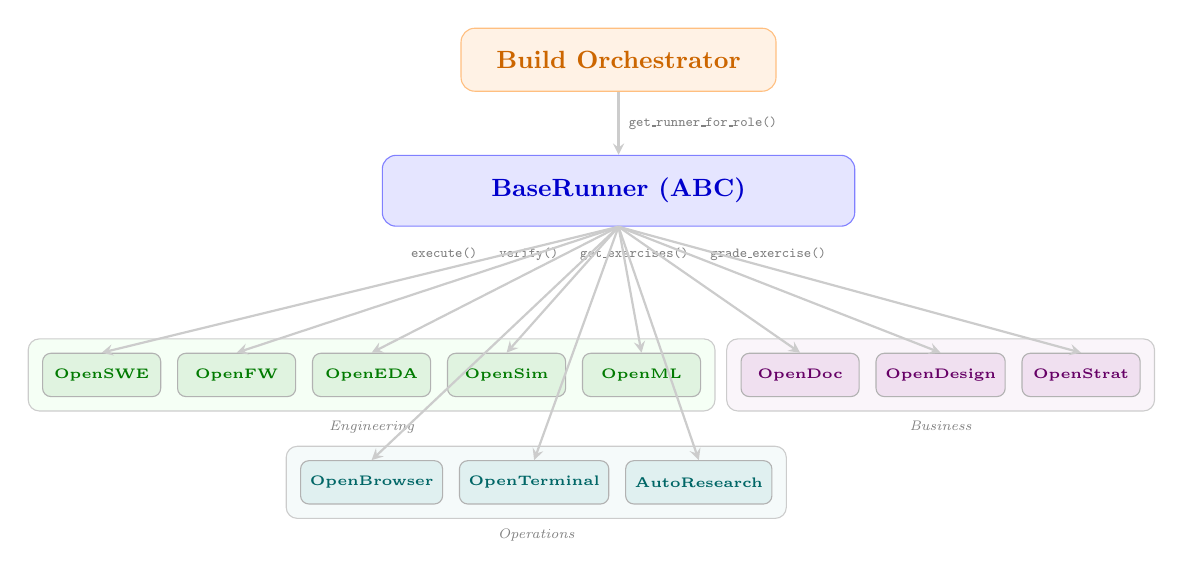
\begin{tikzpicture}[
    base/.style={rectangle, draw=blue!50, rounded corners=5pt, minimum width=6cm, minimum height=0.9cm, font=\small\bfseries, fill=blue!10, text=blue!80!black},
    grp/.style={rectangle, draw=gray!40, rounded corners=4pt, inner sep=5pt, fill=#1!4},
    grp/.default=green,
    runner/.style={rectangle, draw=gray!60, rounded corners=3pt, minimum width=1.5cm, minimum height=0.55cm, font=\tiny\bfseries, fill=#1!12, text=#1!80!black},
    runner/.default=green,
    arr/.style={->, thick, >=stealth, color=gray!40},
    node distance=0.2cm
]
    % Orchestrator at top
    \node[rectangle, draw=orange!50, rounded corners=5pt, fill=orange!10, font=\small\bfseries, text=orange!80!black, minimum width=4cm, minimum height=0.8cm] (orch) {Build Orchestrator};

    % BaseRunner
    \node[base, below=0.8cm of orch] (base) {BaseRunner (ABC)};
    \node[below=0.15cm of base, font=\tiny\ttfamily, text=gray] {execute() \quad verify() \quad get\_exercises() \quad grade\_exercise()};

    \draw[arr] (orch) -- node[right, font=\tiny, color=gray] {\texttt{get\_runner\_for\_role()}} (base);

    % Row 1: Engineering (5 runners)
    \node[runner=green!60!black, below left=1.6cm and 2.8cm of base] (swe) {OpenSWE};
    \node[runner=green!60!black, right=0.2cm of swe]  (fw)  {OpenFW};
    \node[runner=green!60!black, right=0.2cm of fw]   (eda) {OpenEDA};
    \node[runner=green!60!black, right=0.2cm of eda]  (sim) {OpenSim};
    \node[runner=green!60!black, right=0.2cm of sim]  (ml)  {OpenML};

    % Row 1: Business (3 runners)
    \node[runner=violet, right=0.5cm of ml]     (doc)      {OpenDoc};
    \node[runner=violet, right=0.2cm of doc]    (design)   {OpenDesign};
    \node[runner=violet, right=0.2cm of design] (strategy) {OpenStrat};

    % Row 2: Operations (3 runners, centered below)
    \node[runner=teal, below=0.8cm of eda]       (browser)  {OpenBrowser};
    \node[runner=teal, right=0.2cm of browser]   (terminal) {OpenTerminal};
    \node[runner=teal, right=0.2cm of terminal]  (research) {AutoResearch};

    % Group backgrounds
    \begin{scope}[on background layer]
        \node[grp=green, fit=(swe)(ml), label={[font=\tiny\itshape, text=gray]below:Engineering}] {};
        \node[grp=violet, fit=(doc)(strategy), label={[font=\tiny\itshape, text=gray]below:Business}] {};
        \node[grp=teal, fit=(browser)(research), label={[font=\tiny\itshape, text=gray]below:Operations}] {};
    \end{scope}

    % Inheritance arrows
    \foreach \r in {swe,fw,eda,sim,ml,doc,design,strategy,browser,terminal,research} {
        \draw[arr] (base.south) -- (\r.north);
    }

\end{tikzpicture}
\caption{Runner architecture. All 11 domain runners implement the \texttt{BaseRunner} interface, grouped by domain family. The Build Orchestrator selects runners via \texttt{get\_runner\_for\_role()}.}
\label{fig:runners}
\end{figure}

\subsection{Runner Catalog}

\begin{table}[h]
\centering
\caption{Eleven domain-aware runners with their role bindings and capabilities.}
\label{tab:runners}
\begin{tabular}{llp{5cm}}
\toprule
\textbf{Runner} & \textbf{Roles} & \textbf{Key Capability} \\
\midrule
OpenSWE & developer, qa\_engineer & 3-tier: external SWE $\rightarrow$ LangGraph $\rightarrow$ LLM \\
OpenFW & firmware\_engineer & Cross-compilation, HAL, binary metrics \\
OpenEDA & pcb\_designer & Schematics, DRC/ERC, Gerber generation \\
OpenSim & hw\_sim\_engineer & SPICE, Verilog, waveform analysis \\
OpenML & data\_scientist & Train, evaluate, experiment tracking \\
OpenDoc & technical\_writer & Compliance documents, cross-references \\
OpenDesign & ux\_designer & Wireframes, accessibility, design tokens \\
OpenStrategy & product\_manager & PRDs, GTM plans, roadmaps \\
OpenBrowser & qa (supplementary) & Real Chromium via gstack, WCAG audits \\
OpenTerminal & terminal\_operator & tmux sessions, marker-based polling \\
AutoResearch & research\_engineer & Hill-climbing experiments, git tracking \\
\bottomrule
\end{tabular}
\end{table}

\subsection{Sandboxed Execution Cascade}

Agent code execution uses a three-tier isolation cascade (Figure~\ref{fig:sandbox}), attempting the most isolated environment first and falling back gracefully.

\begin{figure}[h]
\centering
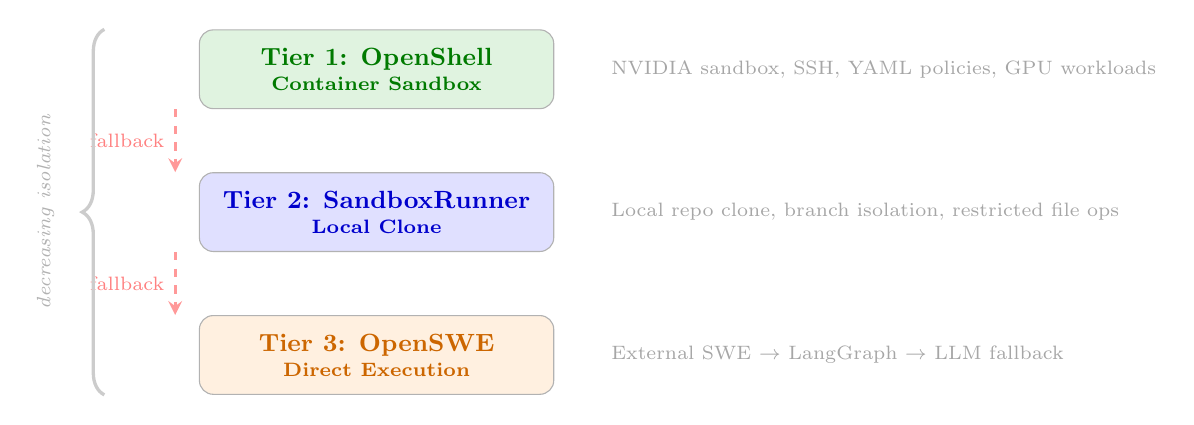
\begin{tikzpicture}[
    tier/.style={rectangle, draw=gray!60, rounded corners=5pt, minimum width=4.5cm, minimum height=1cm, font=\small\bfseries, fill=#1!12, text=#1!80!black, align=center},
    tier/.default=blue,
    desc/.style={font=\scriptsize, text=gray!70, align=left, anchor=west},
    fail/.style={->, very thick, >=stealth, dashed, color=red!40},
    node distance=0.8cm
]
    \node[tier=green!60!black] (t1) {Tier 1: OpenShell\\[-2pt]{\scriptsize Container Sandbox}};
    \node[tier=blue,  below=of t1] (t2) {Tier 2: SandboxRunner\\[-2pt]{\scriptsize Local Clone}};
    \node[tier=orange, below=of t2] (t3) {Tier 3: OpenSWE\\[-2pt]{\scriptsize Direct Execution}};

    % Right-side descriptions
    \node[desc, right=0.6cm of t1.east] {NVIDIA sandbox, SSH, YAML policies, GPU workloads};
    \node[desc, right=0.6cm of t2.east] {Local repo clone, branch isolation, restricted file ops};
    \node[desc, right=0.6cm of t3.east] {External SWE $\rightarrow$ LangGraph $\rightarrow$ LLM fallback};

    % Fallback arrows
    \draw[fail] ([xshift=-0.3cm]t1.south west) -- node[left, font=\scriptsize, color=red!50] {fallback} ([xshift=-0.3cm]t2.north west);
    \draw[fail] ([xshift=-0.3cm]t2.south west) -- node[left, font=\scriptsize, color=red!50] {fallback} ([xshift=-0.3cm]t3.north west);

    % Isolation gradient brace
    \draw[decorate, decoration={brace, amplitude=8pt, mirror}, very thick, color=gray!40]
        ([xshift=-1.2cm]t1.north west) -- ([xshift=-1.2cm]t3.south west)
        node[midway, left=0.5cm, font=\scriptsize\itshape, color=gray!60, rotate=90, anchor=south] {decreasing isolation};
\end{tikzpicture}
\caption{Three-tier sandboxed execution cascade. The orchestrator tries the most isolated tier first and falls back on unavailability. Dashed arrows indicate fallback paths.}
\label{fig:sandbox}
\end{figure}

% ============================================================================
\section{Communication Layers}
\label{sec:communication}

SAGE implements two communication layers for observability and structured messaging (Figure~\ref{fig:comms}).

\begin{figure}[h]
\centering
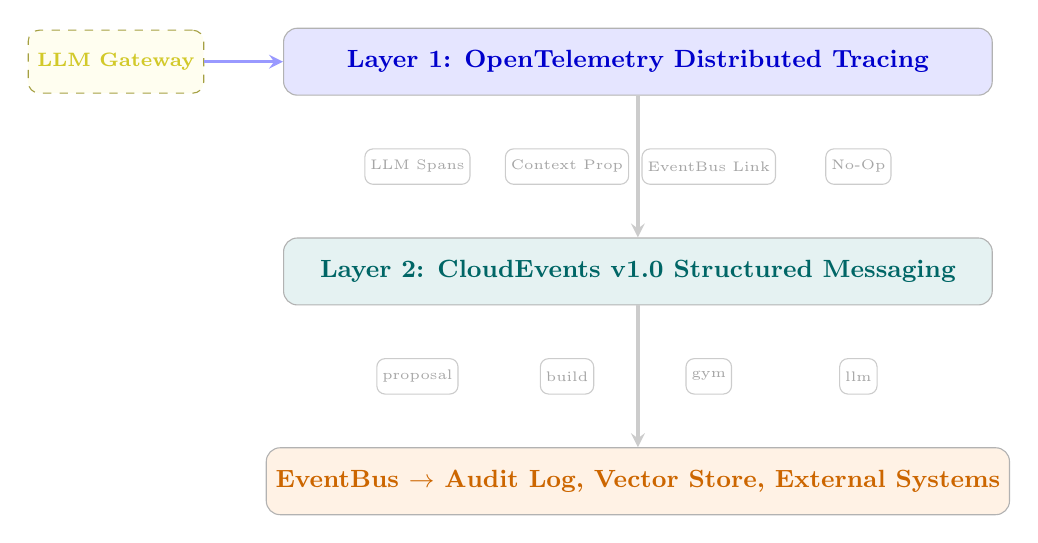
\begin{tikzpicture}[
    layer/.style={rectangle, draw=gray!60, rounded corners=5pt, minimum width=9cm, minimum height=0.85cm, font=\small\bfseries, fill=#1!10, text=#1!80!black},
    layer/.default=blue,
    comp/.style={rectangle, draw=gray!40, rounded corners=3pt, minimum height=0.45cm, font=\tiny, fill=white, text=gray!70, inner sep=2pt},
    arr/.style={->, very thick, >=stealth, color=gray!40},
    node distance=0.5cm
]
    % Layer 1 (centered, no gateway offset)
    \node[layer=blue] (otel) {Layer 1: OpenTelemetry Distributed Tracing};

    % LLM Gateway — source (to the left)
    \node[rectangle, draw=yellow!60!black, dashed, rounded corners=4pt, fill=yellow!6, font=\scriptsize\bfseries, align=center, text=yellow!80!black, minimum height=0.8cm, left=1cm of otel] (gw) {LLM Gateway};

    % Layer 2
    \node[layer=teal, below=1.8cm of otel] (ce) {Layer 2: CloudEvents v1.0 Structured Messaging};

    % Consumers
    \node[layer=orange, below=1.8cm of ce] (consumers) {EventBus $\rightarrow$ Audit Log, Vector Store, External Systems};

    % Layer 1 components — positioned between layer 1 and layer 2
    \path (otel.south) -- (ce.north) coordinate[midway] (mid12);
    \node[comp] at ([xshift=-2.8cm]mid12) (spans) {LLM Spans};
    \node[comp] at ([xshift=-0.9cm]mid12) (ctx) {Context Prop};
    \node[comp] at ([xshift=0.9cm]mid12) (ebus) {EventBus Link};
    \node[comp] at ([xshift=2.8cm]mid12) (noop) {No-Op};

    % Layer 2 components — positioned between layer 2 and consumers
    \path (ce.south) -- (consumers.north) coordinate[midway] (mid23);
    \node[comp] at ([xshift=-2.8cm]mid23) (prop) {proposal};
    \node[comp] at ([xshift=-0.9cm]mid23) (build) {build};
    \node[comp] at ([xshift=0.9cm]mid23) (gymev) {gym};
    \node[comp] at ([xshift=2.8cm]mid23) (llmev) {llm};

    % Connections
    \draw[arr, color=blue!40] (gw) -- (otel);
    \draw[arr] (otel) -- (ce);
    \draw[arr] (ce) -- (consumers);

\end{tikzpicture}
\caption{Communication layers. Layer~1 provides distributed tracing with graceful no-op degradation. Layer~2 wraps domain events in CloudEvents v1.0 envelopes. Both feed into the EventBus for pub/sub distribution.}
\label{fig:comms}
\end{figure}

\subsection{Layer 1: OpenTelemetry Distributed Tracing}

The tracing module (\texttt{src/core/tracing.py}) provides OpenTelemetry integration with graceful degradation. When the OpenTelemetry SDK is absent, all tracing functions operate as no-ops via stub classes (\texttt{\_NoOpSpan}, \texttt{\_NoOpTracer}), ensuring zero impact on calling code.

Key capabilities:
\begin{itemize}[noitemsep]
    \item Span creation with GenAI semantic conventions on every \texttt{generate()} call
    \item Cross-process context propagation via carrier dictionaries
    \item EventBus span linkage for event-driven architectures
    \item Thread-safe tracer initialization with caching
\end{itemize}

\subsection{Layer 2: CloudEvents v1.0 Envelope}

The CloudEvents module (\texttt{src/modules/cloud\_events.py}) implements the CloudEvents v1.0 specification~\citep{cloudevents2024} as a zero-dependency Python dataclass. Typed factory functions (\texttt{proposal\_event}, \texttt{build\_event}, \texttt{gym\_event}, \texttt{llm\_event}) ensure consistent event creation. Events integrate with the existing EventBus for pub/sub distribution.

% ============================================================================
\section{Modular Skill Marketplace}
\label{sec:skills}

Skills are YAML files defining agent capabilities with runner bindings, role mappings, grading rubrics, and certification requirements. The skill system supports three visibility tiers:

\begin{itemize}[noitemsep]
    \item \textbf{Public} --- open-source skills shipped with SAGE (17 skills across 10+ domains)
    \item \textbf{Private} --- proprietary skills loaded via \texttt{SAGE\_SKILLS\_DIR} environment variable, never committed to the open-source repository
    \item \textbf{Disabled} --- dormant skills retained for versioning but not loaded
\end{itemize}

Skills are hot-reloadable at runtime without server restart. Each skill defines acceptance criteria and grading rubrics used by the Agent Gym for automated evaluation.

% ============================================================================
\section{Connector Framework}
\label{sec:connectors}

SAGE provides a pluggable connector architecture for integrating external data sources into the agent knowledge pipeline. Inspired by the Onyx project's approach to unified data ingestion, the framework defines an abstract base connector with three required methods: \texttt{connect()}, \texttt{fetch()}, and \texttt{sync()}.

\subsection{Architecture}

The \texttt{ConnectorRegistry} implements the registry pattern: connectors self-register at import time, and the API layer discovers available types dynamically. This enables adding new data sources without modifying existing code.

\begin{lstlisting}[language=Python, caption={BaseConnector abstract interface.}]
class BaseConnector(ABC):
    @abstractmethod
    def connect(self, config: dict) -> bool: ...
    @abstractmethod
    def fetch(self, query: str) -> list[dict]: ...
    @abstractmethod
    def sync(self) -> dict: ...
\end{lstlisting}

\subsection{Shipped Connectors}

Two connectors ship with the framework:

\begin{itemize}[noitemsep]
    \item \textbf{GitHub Connector} --- uses the \texttt{gh} CLI to fetch issues, pull requests, and commits from configured repositories. Requires no API key when \texttt{gh} is authenticated.
    \item \textbf{Filesystem Connector} --- indexes local text files by extension (26 supported extensions), respecting configurable \texttt{max\_files} and \texttt{max\_size} limits.
\end{itemize}

API endpoints: \texttt{GET /connectors} (list available types), \texttt{POST /connectors/\{type\}/configure}, \texttt{POST /connectors/\{type\}/sync}.

% ============================================================================
\section{Complexity-Based Model Routing}
\label{sec:routing}

To optimize cost without sacrificing quality, SAGE implements heuristic complexity classification that routes prompts to cost-appropriate LLM providers.

\subsection{Classification}

The \texttt{ComplexityClassifier} scores prompts on a 0--100 scale across four dimensions:

\begin{table}[h]
\centering
\small
\caption{Complexity scoring dimensions.}
\label{tab:complexity}
\begin{tabular}{@{}llc@{}}
\toprule
\textbf{Dimension} & \textbf{Signal} & \textbf{Max Points} \\
\midrule
Length        & Word count thresholds (20/50/100/200+) & 40 \\
Code blocks  & Presence of \texttt{```} fenced blocks    & 20 \\
Tool keywords & \texttt{implement}, \texttt{refactor}, \texttt{debug}, etc. & 25 \\
Safety domain & \texttt{FMEA}, \texttt{ASIL}, \texttt{IEC 62304}, etc.      & 20 \\
\bottomrule
\end{tabular}
\end{table}

Thresholds: LOW ($<15$), MEDIUM (15--45), HIGH ($>45$). The \texttt{route\_to\_model()} function maps complexity to provider tiers (e.g., LOW $\rightarrow$ Haiku/Flash, MEDIUM $\rightarrow$ Sonnet, HIGH $\rightarrow$ Opus/Pro).

\subsection{Integration}

Classification runs inside \texttt{LLMGateway.generate()} after PII detection and before budget checks. Routing statistics are exposed via \texttt{GET /llm/routing-stats} and displayed in the Costs dashboard with color-coded LOW/MEDIUM/HIGH counters.

% ============================================================================
\section{Persistent Stores}
\label{sec:stores}

Two SQLite-backed stores provide server-side persistence for data previously held only in browser localStorage:

\begin{itemize}[noitemsep]
    \item \textbf{Chat Store} (\texttt{chat\_conversations} table) --- persists conversation history with role context, enabling cross-device access and surviving browser data clears. Fields: id, user\_id, solution, role\_id, role\_name, title, messages (JSON), timestamps.
    \item \textbf{Goals Store} (\texttt{objectives} table) --- persists OKR objectives and key results with quarter-based filtering. Fields: id, user\_id, solution, title, quarter, status, owner, key\_results (JSON), timestamps.
\end{itemize}

Both stores use WAL mode with busy timeouts for concurrent access safety. The frontend uses TanStack Query (\texttt{useQuery}/\texttt{useMutation}) with graceful fallback to localStorage when the API is unreachable.

% ============================================================================
\section{Best-First Tree Search}
\label{sec:bfts}

Inspired by the AI-Scientist-v2 approach to solution-space exploration~\citep{aiscientistv2}, the Agent Gym integrates a Best-First Tree Search (BFTS) evaluator for candidate solution ranking and refinement.

\subsection{Algorithm}

Given $N$ candidate solutions, the evaluator:
\begin{enumerate}[noitemsep]
    \item Scores all candidates via a configurable scorer function
    \item Sorts the frontier by score (descending) --- best-first expansion
    \item Expands top-$k$ nodes by generating $b$ child variants per node (branching factor)
    \item Repeats until \texttt{max\_depth} or \texttt{max\_iterations} is reached
    \item Returns the highest-scoring node across the entire search tree via DFS
\end{enumerate}

\begin{equation}
\text{best} = \arg\max_{n \in \text{tree}} \text{scorer}(n.\text{solution})
\label{eq:bfts}
\end{equation}

The search is exposed via \texttt{POST /gym/tree-search} with configurable \texttt{max\_depth} (default 3), \texttt{branching\_factor} (default 3), and \texttt{max\_iterations} (default 50). In production, the scorer function would be an LLM-based evaluator; the default implementation uses a length-based heuristic for testing.

% ============================================================================
\section{Evaluation}
\label{sec:evaluation}

We evaluate SAGE across two dimensions: agent skill development via the Agent Gym, and end-to-end product construction via the Build Orchestrator.

\subsection{Agent Gym Training Results}

\begin{table}[h]
\centering
\caption{Agent Gym training results: 618 sessions across 33 skill-role combinations. Combinations with $<10$ sessions are marked with $\dagger$.}
\label{tab:gym-results}
\begin{tabular}{llcccc}
\toprule
\textbf{Agent Role} & \textbf{Skill} & \textbf{Rating ($\mu$)} & \textbf{RD ($\phi$)} & \textbf{Sessions} & \textbf{Win Rate} \\
\midrule
developer & agentic\_eng.$\dagger$ & 1691 & 171 & 5 & 100\% \\
agentic\_engineer & agentic\_eng. & 1660 & 117 & 13 & 77\% \\
ml\_engineer & gen\_ai\_eng. & 1620 & 92 & 24 & 58\% \\
ml\_engineer & machine\_learning & 1610 & 84 & 31 & 68\% \\
developer & software\_eng. & 1585 & 115 & 15 & 80\% \\
\midrule
\multicolumn{2}{l}{\textit{Average across all 33 combinations}} & 1484 & --- & 15 & --- \\
\midrule
analyst & technical\_writing & 1273 & 98 & 19 & 16\% \\
embedded\_tester & firmware\_eng. & 1339 & 102 & 19 & 32\% \\
marketing\_strat. & product\_strategy & 1347 & 95 & 19 & 32\% \\
\bottomrule
\end{tabular}
\end{table}

\textbf{Key findings:}
\begin{itemize}[noitemsep]
    \item 100\% of agent-skill combinations reached the deployment-readiness threshold ($\phi < 200$), though combinations with fewer than 10 sessions (marked $\dagger$) should be interpreted with caution.
    \item 76\% achieved confident deployment ($\phi < 150$).
    \item Engineering-domain agents significantly outperform non-technical agents ($\mu = 1691$ vs.\ $\mu = 1273$). This 418-point gap likely reflects fundamental LLM capability boundaries: code generation is more structured and verifiable than open-ended strategic tasks.
    \item Spaced repetition scheduling improved retention of previously failed exercises.
\end{itemize}

\subsection{100-Solution Stress Test}

We evaluated the Build Orchestrator on 100 product descriptions spanning 10 industry domains (10 per domain).

\begin{table}[h]
\centering
\caption{100-solution pipeline stress test results.}
\label{tab:pipeline}
\begin{tabular}{lc}
\toprule
\textbf{Outcome} & \textbf{Count} \\
\midrule
End-to-end success & 2 \\
Planner decomposition failure & 19 \\
Incomplete (timeout/resource) & 80 \\
Error & 1 \\
\bottomrule
\end{tabular}
\end{table}

\textbf{Root causes:}
\begin{enumerate}[noitemsep]
    \item \textbf{Context overflow} --- complex product descriptions exceeded context windows during decomposition
    \item \textbf{Critic revision degradation} --- plan quality dropped across iterations (52 $\rightarrow$ 34 $\rightarrow$ 21) before context-aware rewrite stabilized at 54 $\rightarrow$ 36 $\rightarrow$ 67
    \item \textbf{LLM latency variance} --- 30--500s per generation call; full builds required 40--70 minutes
    \item \textbf{Anti-drift warnings} --- 39 quality drift events in a single 3-domain run
\end{enumerate}

The 2\% success rate demonstrates the architecture's end-to-end viability while honestly exposing the significant prompt engineering and context management work required for production-scale deployment.

\subsection{Test Infrastructure}

\begin{table}[h]
\centering
\caption{Test suite coverage.}
\label{tab:tests}
\begin{tabular}{lcc}
\toprule
\textbf{Suite} & \textbf{Tests} & \textbf{Pass Rate} \\
\midrule
Framework unit tests (97 files) & 1,569+ & 100\% \\
E2E system tests & 58 & 100\% \\
Agent Gym system tests & 48 & 100\% \\
Browser E2E tests (7 spec files) & 93 & 100\% \\
Frontend unit tests (11 files) & 45+ & 100\% \\
\bottomrule
\end{tabular}
\end{table}

% ============================================================================
\section{Discussion}
\label{sec:discussion}

\subsection{Strengths}

SAGE occupies a unique position at the intersection of open-source, compliance-first, multi-domain, and agent training capabilities. The YAML-first configuration model enables new industry adoption without code changes, validated across 19 bundled solution templates spanning medical devices, automotive, aerospace, fintech, and IoT.

The compounding memory architecture --- where every human approval and rejection enriches future agent context --- provides measurable improvement without model retraining. This follows the Memento principle~\citep{memento2025}: behavioral optimization via memory retrieval, decoupled from the underlying LLM.

\subsection{Limitations}

\textbf{Build Orchestrator scaling.} The 2\% success rate on the 100-solution test is the most significant limitation. Root causes are well-understood (context overflow, critic degradation), but closing the gap to commercial viability (target: 50\%+) requires substantial prompt engineering and possibly architectural changes to context management.

\textbf{Non-technical agent performance.} The 418-point Glicko-2 gap between top engineering agents ($\mu = 1691$) and bottom non-technical agents ($\mu = 1273$) may reflect fundamental LLM capability boundaries rather than addressable prompt engineering deficits. Code generation is inherently more verifiable (compile, test, execute) than strategic advice.

\textbf{No production deployment.} All evaluation was performed in development environments. Production validation in regulated organizations with real compliance audits remains future work.

\textbf{Single-developer origin.} The initial system was developed by one engineer over 16 days (194 commits). While this demonstrates achievable velocity, bus factor 1 is a real concern for production adoption. Open-sourcing the codebase is a deliberate step toward mitigating this risk.

\subsection{Threats to Validity}

\textbf{Internal validity.} Agent Gym ratings depend on the quality of grading rubrics and critic prompts. Biased rubrics would produce misleading ratings. We mitigate this by using N-provider multi-critic review (aggregating scores from multiple independent LLMs), but the rubrics themselves have not been externally validated.

\textbf{External validity.} All 618 training sessions used a single primary LLM provider. Results may not generalize to other providers. The 100-solution stress test used descriptions authored by the development team, which may not represent the diversity of real-world product descriptions.

\textbf{Construct validity.} The Glicko-2 rating system was designed for competitive games (chess, Go), not for agent skill assessment. While the mathematical properties (uncertainty quantification, volatility tracking) are useful, the interpretation of rating differences in this context is not established. A 100-point gap in chess corresponds to approximately 64\% expected win rate; the analogous interpretation for agent skills is undefined.

\textbf{Reproducibility.} LLM outputs are non-deterministic. Running identical training sessions will produce different ratings. We do not currently set random seeds or control for temperature, which limits exact reproducibility. The aggregate trends (engineering $>$ non-technical, spaced repetition helps) are expected to reproduce, but specific ratings will vary.

\subsection{Comparison to Existing Frameworks}

\begin{table}[h]
\centering
\caption{Feature comparison with existing frameworks for regulated environments. \checkmark = full support, $\sim$ = partial support, -- = not supported.}
\label{tab:comparison}
\begin{tabular}{lccccc}
\toprule
\textbf{Capability} & \textbf{SAGE} & \textbf{LangGraph} & \textbf{CrewAI} & \textbf{AutoGen} & \textbf{Dify} \\
\midrule
Mandatory HITL & \checkmark & $\sim$ & -- & -- & $\sim$ \\
Immutable audit & \checkmark & -- & -- & -- & $\sim$ \\
Trace IDs & \checkmark & -- & -- & -- & -- \\
Rejection feedback & \checkmark & -- & -- & -- & -- \\
YAML-only domains & \checkmark & -- & $\sim$ & -- & $\sim$ \\
Zero API keys & \checkmark & $\sim$ & $\sim$ & $\sim$ & -- \\
Build orchestrator & \checkmark & -- & -- & -- & -- \\
Agent training & \checkmark & -- & -- & -- & -- \\
Domain runners & \checkmark & -- & -- & -- & -- \\
\bottomrule
\end{tabular}
\end{table}

LangGraph provides optional \texttt{interrupt\_before} for human intervention ($\sim$); Dify has workflow-level approval gates ($\sim$) and basic logging ($\sim$). CrewAI supports YAML role definitions ($\sim$) and Dify has a UI-based configuration ($\sim$).

% ============================================================================
\section{Conclusion}
\label{sec:conclusion}

SAGE demonstrates that governance-first multi-agent orchestration is architecturally viable for regulated industries. The two-tier governance model, compounding memory architecture, and domain-aware runner system provide the structural guarantees that compliance-bound organizations require.

The honest assessment is that SAGE is early-stage. The Build Orchestrator works end-to-end but fails at scale. Non-technical agents underperform. There are zero production deployments. However, the market gap is real --- no competing framework provides mandatory human governance with immutable audit trails and domain-agnostic configuration. The EU AI Act and FDA AI/ML guidance are creating regulatory demand that will only grow.

Future work includes: (1)~improving Build Orchestrator success rate to 50\%+ through context management and prompt engineering; (2)~hardening three priority domain runners (OpenSWE, OpenML, OpenDoc) to production quality; (3)~conducting first pilot deployments in regulated organizations; (4)~scaling the Agent Gym exercise catalog to validate the variant generation pipeline at 10,000+ exercises; (5)~expanding the Connector Framework with Slack webhook and Jira connectors; and (6)~validating complexity-based routing cost savings across diverse workloads.

SAGE is available under the MIT License at \url{https://github.com/Sumanharapanahalli/SAGE}.

% ============================================================================
\section*{Acknowledgments}

The architectural design of SAGE was influenced by several open-source projects and research efforts: LangGraph for graph-based orchestration patterns, DeerFlow~\citep{deerflow2025} (ByteDance) for supervisor-agent topology, Paperclip for governance models, Aider for git-integrated code changes, Claude Code for project-level runtime directories, AI-Scientist-v2~\citep{aiscientistv2} for BFTS tree search, Onyx for connector-based data ingestion, and the Meta-Harness paper (arXiv:2603.28052) for terminal execution innovations.

% ============================================================================
\bibliographystyle{plainnat}
\bibliography{sage}

\end{document}
